\section{Stream Ciphers}
A \textbf{stream cipher} operates on one plaintext symbol at a time and use generator function to create pseudo-random keystream. Ideally, we should use a \textit{true random number generator} (TRNG), but they are usually slow, for this reason we use \textit{pseudo-random number generator} (PRNG). A PRNG should have \textit{forward and backward unpredictability}. Let's see some famous PRNGs.
\subsection{Linear Congruential Generator}
The random number sequence $\{X_n\}$ is obtained as $X_{n+1} = (a\cdot X_n + c) \Mod{m}$
It goes without saying that in this case the selection of values for $(a,c,m)$ is critical in developing a good PRNG.
\subsection{Blum Blum Shub (BBS) Generator}
One of the most commonly used PRNGs. The random number sequence $\{X_n\}$ is obtained as follow
\begin{enumerate}
    \item Choose two prime $(p,q)$ s.t. $p\equiv q\equiv 3 \Mod{4}$
    \item Let $n=p\times q$
    \item Choose random $s$ such that $\texttt{gcd}(s,n)=1$
    \item Start from $X_0=s^2 \Mod{n}$
    \item If we want $n$ bits, we repeat $n$ times the following
    \begin{enumerate}
        \item Compute $X_i=(X_{i-1})^2 \Mod{n}$
        \item Take only the LSB from $X_i$
    \end{enumerate}
\end{enumerate}

\subsection{PRNGs using block modes}
\begin{wrapfigure}{r}{0.3\textwidth}
\vspace{-65pt}
\fbox{
\begin{center}
    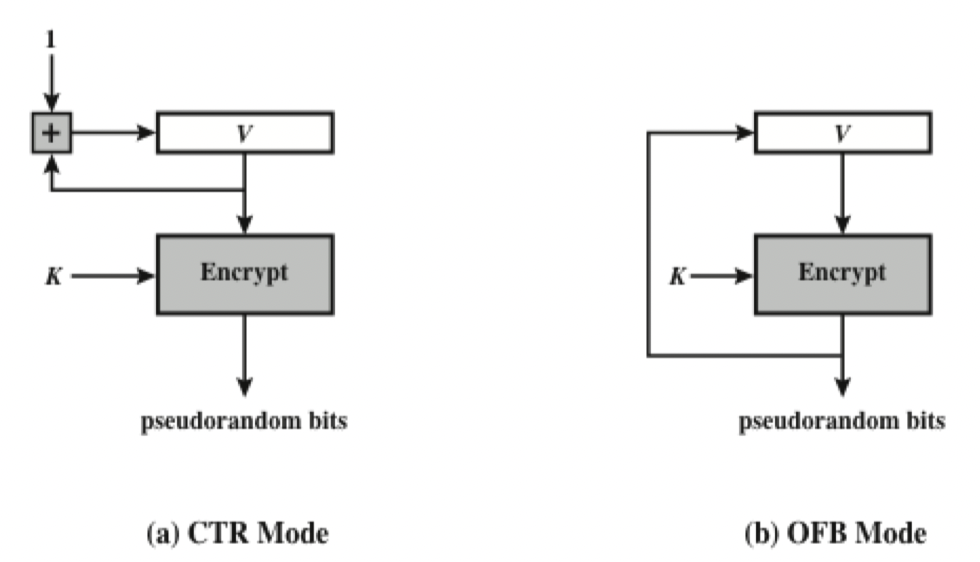
\includegraphics[scale=0.3]{images/prng.png}
\end{center}}
\end{wrapfigure}
It is also possible to create a PRNG starting from a CTR or an OFB mode: they just need a key $K$ and an initial vector $V_0$ (that can be fix, e.g. $V_0=0$)

\subsection{RC4}
RC4 is a variable key size stream cipher. To generate the key stream, the cipher makes use of a secret internal state which consists of two parts:
\begin{itemize}
    \item A permutation of all 256 possible bytes ($S$)
    \item Two 8-bit index-pointers ($i$ and $j$).
\end{itemize}
The permutation is initialized with a variable length key using the key-scheduling algorithm (KSA). Then the stream of bits is generated by a pseudo-random generation algorithm.
\begin{center}
    \fbox{
    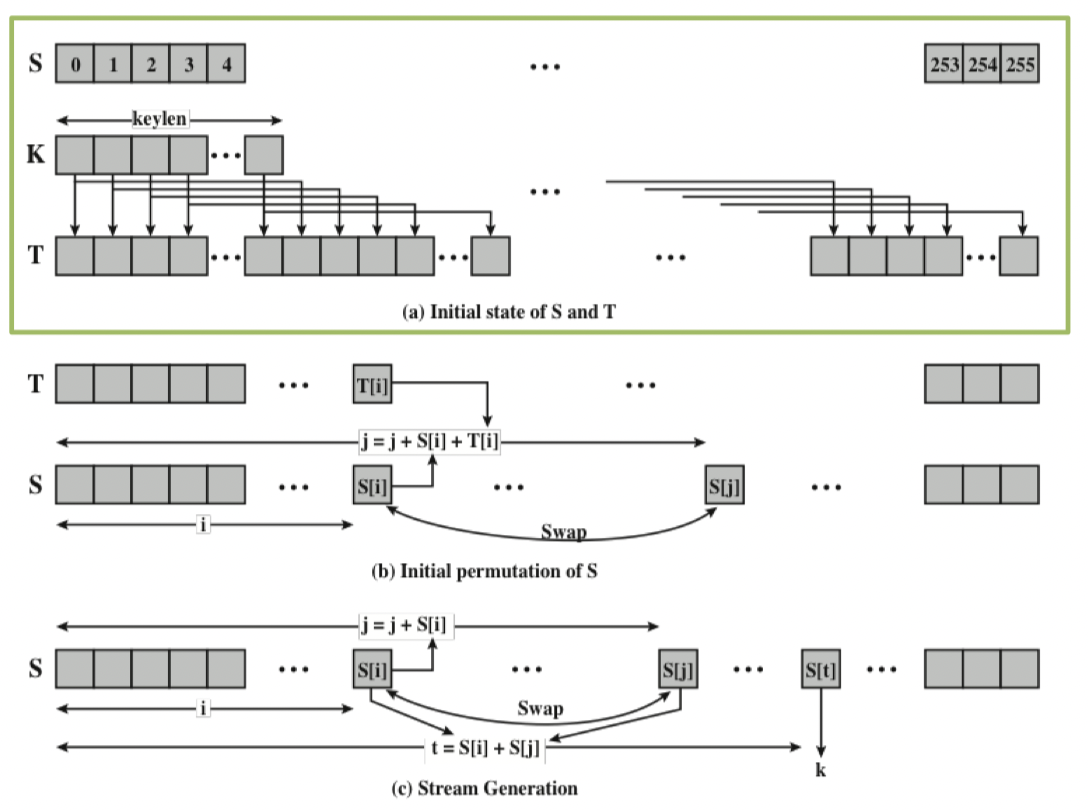
\includegraphics[scale=0.7]{images/rc4.png}}
\end{center}
